\documentclass{article}
\usepackage[utf8]{inputenc}
\usepackage[spanish, es-tabla]{babel}
\usepackage{amsmath,amsfonts,amssymb,amsthm,float,bbm}
\usepackage{graphicx}

\author{Jorge Carlos Urteaga \and Víctor R. Martinez}
\title{Aprendizaje de Máquina \\ Projecto Final}
\date{\today}
\decimalpoint

\usepackage{Sweave}
\begin{document}
\Sconcordance{concordance:Final.tex:Final.Rnw:%
1 11 1 1 0 4 1 1 23 12 1 1 4 6 0 1 2 2 1 1 3 2 0 1 2 4 0 1 2 1 1 1 3 6 %
0 1 2 3 1 1 12 70 0 1 1 6 0 1 2 4 1 1 13 12 0 1 1 1 4 3 0 1 4 7 0 1 2 4 %
1 1 3 2 0 1 2 1 0 1 1 1 5 8 0 1 2 2 1 1 6 5 0 3 1 1 2 1 0 1 1 3 0 1 2 2 %
1 1 12 11 0 1 1 1 4 3 0 1 2 5 0 1 2 9 1}


\maketitle

\section{Introducción}
???

\section{Datos}
???

\section{Procesamiento de los datos}

\subsection{Inicialización}
El siguiente código importa las librerías a utilizar, lee los datos del archivo de datos y genera los indices para la validación cruzada de 5 iteraciones (\emph{k-folds cross validation})
\begin{Schunk}
\begin{Sinput}
> library(ggplot2)
> library(e1071)
> library(plyr)
> library(reshape2)
> library(nnet)
> library(randomForest)
> set.seed(107346)
> alacranes <- read.csv("csvlist1.csv")
> alacranes[which(alacranes$tipo == 1111), c("tipo")] <- 0
> alacranes[which(alacranes$tipo == 2222), c("tipo")] <- 1
> alacranes$tipo <- as.factor(alacranes$tipo)
> #Quitamos la columna ID
> alacranes <- alacranes[,!names(alacranes) %in% c("ID")]
> #Creacion de las folds
> obs <- sample(seq(1, dim(alacranes)[1]),dim(alacranes)[1], replace=F)
> max <- length(obs)/5
> kfolds <- split(obs, ceiling(seq_along(obs)/max))
> #Cuadricula para dibujar las componentes
> dat.x <- expand.grid(Comp.1 = seq(-30,30,0.5),
+                      Comp.2 = seq(-20,20,0.5))
\end{Sinput}
\end{Schunk}

En primer lugar los datos fueron escalados y centrados a media $0$ y varianza $1$ para eliminar el ruido producto de utilizar diferentes unidades entre las variables y para reducir la dimensión del espacio de variables utilizando PCA.

\begin{Schunk}
\begin{Sinput}
> #Escalamos las variables a mu = 0, sigma = 1
> alacranes.scaled <- data.frame(scale(alacranes[,-141]),
+                                tipo = alacranes$tipo)
\end{Sinput}
\end{Schunk}

A continuación, reducimos la dimensionalidad del problema utilizando un Análisis de Componentes Principales. Encontramos que con sólo 40 factores eramos capaces de capturar el 97.397\% de la varianza de los datos.

\begin{Schunk}
\begin{Sinput}
> pca <- princomp(~., data=alacranes.scaled[, -141],
+                 cor = TRUE, na.action=na.exclude)
> datos.red <- data.frame(pca$scores[,1:40],
+                         tipo = alacranes.scaled$tipo)
\end{Sinput}
\end{Schunk}

A partir de los componentes más importantes, podemos representar nuestro problema en dos dimensiones para una mejor interpretación de los datos y una primera aproximación al procedimiento que tendremos que utilizar. Como podemos ver en la siguiente figura, los alacranes no venenosos se encuentran agrupados en el centro de los datos rodeados por alacranes venenosos. Es claro que un modelo lineal sería incapaz de separar de manera adecuada los datos, necesitamos un modelo capaz de generar áreas de clasificación circulares.
\begin{Schunk}
\begin{Sinput}
> ggplot(aes(x = Comp.1, y = Comp.2, color = tipo),
+        data = datos.red) + geom_point() + xlim(-30, 30) + ylim(-20, 20)
\end{Sinput}
\end{Schunk}
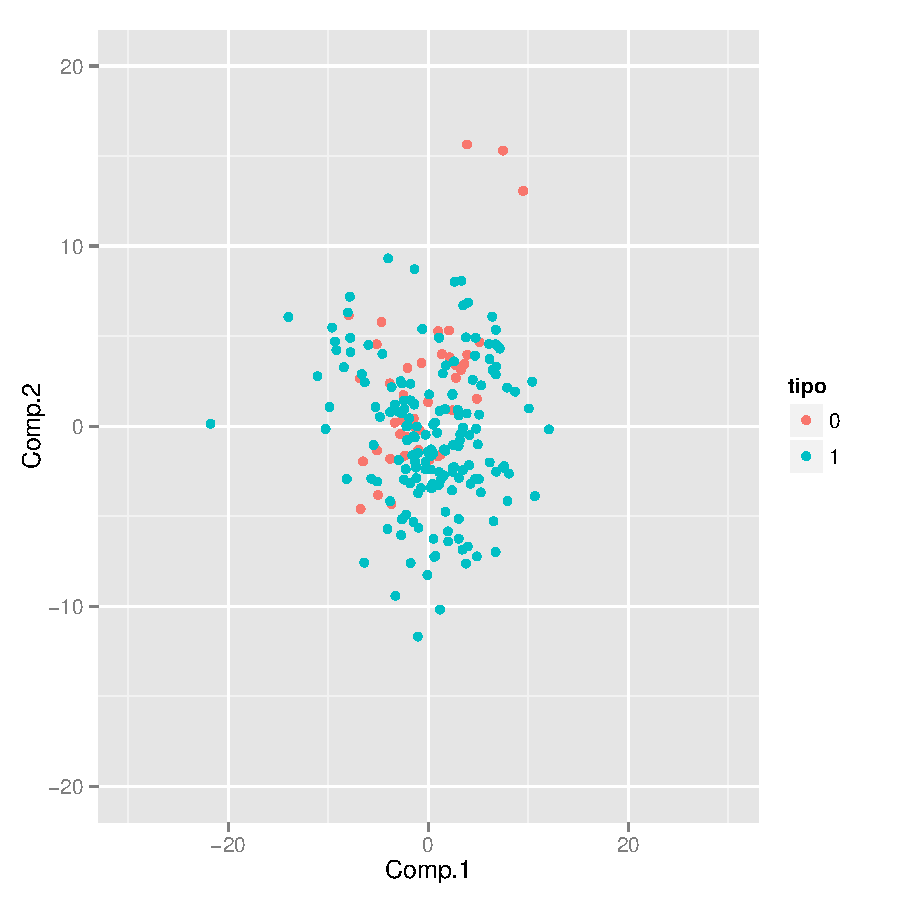
\includegraphics{Final-004}

\section{Métodos}
\subsection{Red neuronal}
Nuestra primera aproximación al problema fue mediante el uso de una red neuronal. Se entrenó una red neuronal con 12 neuronas en la capa escondida (número determinado de manera empírica) con decaimiento ($10^{-9}$) en un máximo de 1000 iteraciones. Para medir el comportamiento de la red, se utilizó un procedimiento de validación cruzada a 5 iteraciones.
\begin{Schunk}
\begin{Sinput}
> ann.cross.validation <- sapply(seq(1,5), function(i){
+   train <- datos.red[unlist(kfolds[c(-i)]),]
+   test <- datos.red[kfolds[[i]],]
+   invisible(capture.output(ann <- nnet(tipo ~ ., data = train, size = 12,
+               decay = 1E-9, maxit = 1000)))
+   preds <- predict(ann, newdata = test)
+   mean(preds == test$tipo)
+ })
> mean(ann.cross.validation)
\end{Sinput}
\begin{Soutput}
[1] 0.7204787
\end{Soutput}
\end{Schunk}
En todas las iteraciones de validación cruzada la red convergió. El resultado final fue decepcionante, ya que la red sólo fue capaz de predecir $72.465\%$ de los casos. Como se verá en la siguiente sección, la máquina de soporte vectorial alcanzó mejores resultados en comparación.

\subsection{Máquina de soporte vectorial}
El segundo método estudiado fueron las máquinas de soporte vectorial. Debido a la forma estudiada de los datos se optó por utilizar un \emph{kernel} de tipo radial, con gamma igual a $2$ (determinado empíricamente). De nueva cuenta recurrimos a la validación cruzada de 5 iteraciones para determinar el mejor parámetro de castigo $C$. El espacio explorado fueron las potencias de 10 desde $-3$ hasta $5$. La siguiente figura muestra el promedio de la certeza del estimado junto con sus barras de error estándar con parámetro $C$ en escala logarítmica. Podemos ver que para $C$ pequeñas, el desempeño del estimador es estadísticamente más bajo que para $C > 1$.

\begin{Schunk}
\begin{Sinput}
> cross.validation <- sapply(c(0.0001, 0.001,0.005, 0.01,0.05,
+                              0.1, 0.5, 1, 2, 3, 5, 10, 50,
+                              100, 250, 500, 1000, 5000,
+                              10000, 15000, 1000000),function(C){
+   medias.C <- sapply(seq(1, 5), function(i){
+     #train <- datos.red[unlist(kfolds[c(-i)]),]
+     #test <- datos.red[kfolds[[i]],]
+     
+     train <- alacranes.scaled[unlist(kfolds[c(-i)]),]
+     test <- alacranes.scaled[kfolds[[i]],]
+     
+     svm.c <- svm(tipo ~ ., data = train, kernel = "radial",
+                  gamma = 2, cost = C)
+     preds <- predict(svm.c, newdata = test)
+     mean(preds == test$tipo)
+   })
+ })
> cross.validation <- t(cross.validation)
> cv.summarize <- data.frame(C = c(0.0001, 0.001,0.005, 0.01,0.05,
+                                  0.1, 0.5, 1, 2, 3, 5, 10, 50,
+                                  100, 250, 500, 1000, 5000,
+                                  10000, 15000, 1000000),
+                            mean = rowSums(cross.validation)/5,
+                            sd = apply(cross.validation, 1, sd))
> max(cv.summarize$mean)
\end{Sinput}
\begin{Soutput}
[1] 0.8687943
\end{Soutput}
\begin{Sinput}
> ggplot(aes(x = log(C), y = mean),
+        data = cv.summarize) + geom_errorbar(aes(ymin = mean -sd,
+                                                 ymax = mean + sd,
+                                                 width=.1)) + geom_point()
\end{Sinput}
\end{Schunk}
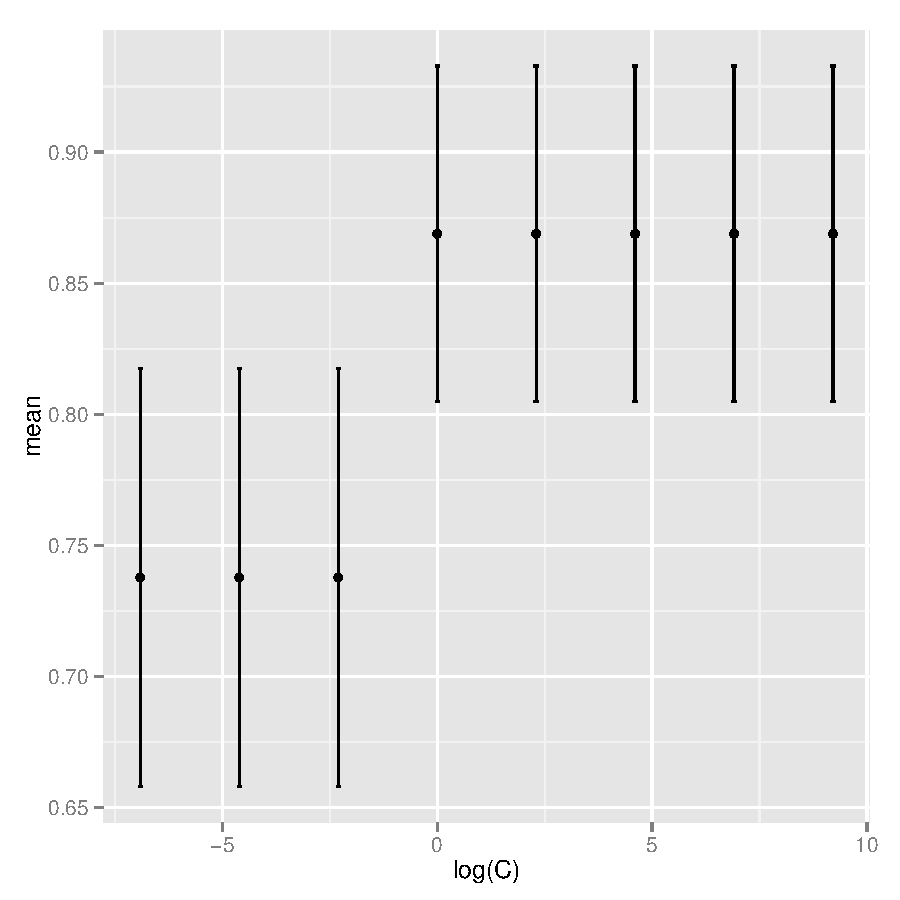
\includegraphics{Final-006}

Para $C > 1$, este clasificador obtuvo una tasa media de clasificación de $86.879\%$ con una desviación estándar de $0.06403$. 

De nueva cuenta, podemos graficar el comportamiento del estimador en dos dimensiones (a partir de los principales factores encontrados). A continuación se muestra como es que el SVM de \emph{kernel} radial con parámetro de castigo $C = 100$ clasifica los puntos del espacio $\mathbb{R}^2$. 

\begin{Schunk}
\begin{Sinput}
> svm.opt <- svm(tipo ~ Comp.1 + Comp.2, data = datos.red,
+                kernel = "radial", gamma = 2, cost = 100)
> dat.x$preds.1 <- predict(svm.opt, newdata = dat.x)
> ggplot(dat.x, aes(x = Comp.1, y = Comp.2, 
+                   colour = preds.1)) + 
+   geom_point(size = 1) +
+   geom_point(aes(x = Comp.1, y = Comp.2,
+                  color = tipo),
+              data = datos.red,
+              size = 3) + xlim(-30, 30) + ylim(-20, 20)
\end{Sinput}
\end{Schunk}
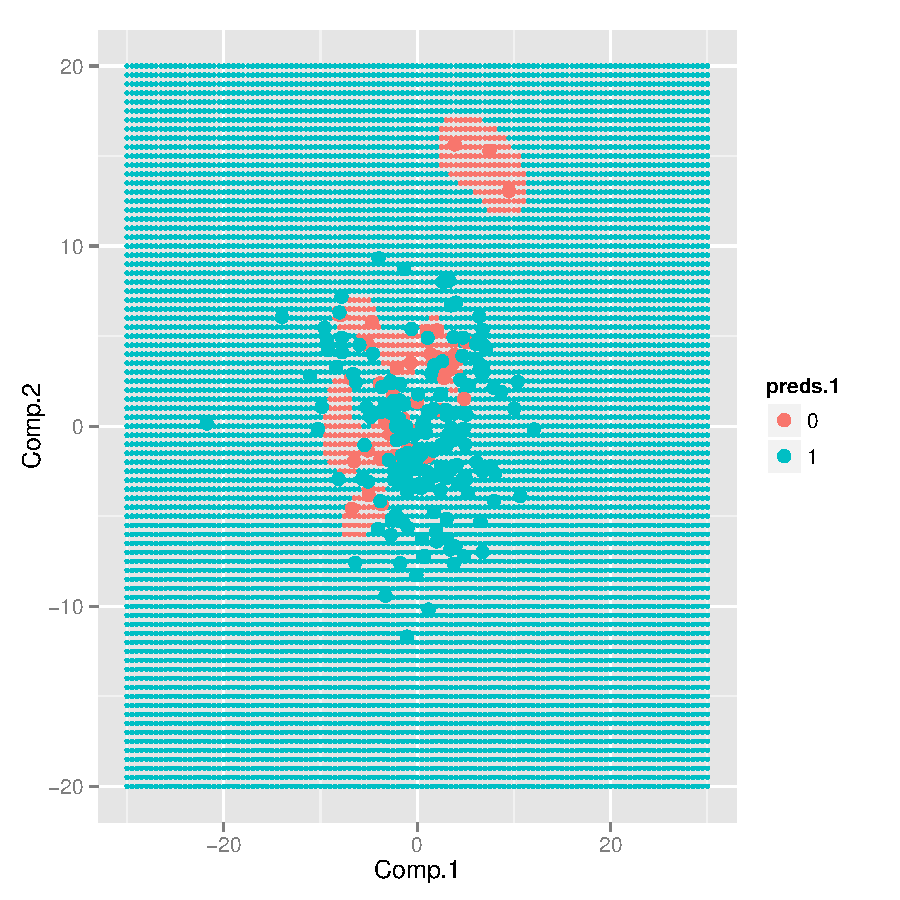
\includegraphics{Final-007}
\subsubsection{Sensibilidad, Precisión y score F1}
Nos interesa saber que tan bueno es el desempeño de nuestro modelo al clasificar una muestra de ejemplos. En primer lugar obtenemos separamos nuestros datos reducidos en una muestra de 80\% entrenamiento y 20\% prueba. Para asegurar que la muestra de entrenamiento tenga tanto muestras positivas como muestras negativas, recurrimos a un proceso de muestreo estratificado donde seleccionamos un subconjunto de cada grupo a clasificar de acuerdo a su tamaño relativo en los datos.

\begin{Schunk}
\begin{Sinput}
> idx.tipo1 <- sample(which(alacranes.scaled$tipo == 1), .8 * 174)
> idx.tipo0 <- sample(which(alacranes.scaled$tipo == 0), .8 * 0.7372881 * 62)
> train <- alacranes.scaled[c(idx.tipo1, idx.tipo0),]
> test <- alacranes.scaled[-c(idx.tipo1, idx.tipo0),]
> #Shuffle data
> train <- train[sample(dim(train)[1]),]
> test <- test[sample(dim(test)[1]),]
\end{Sinput}
\end{Schunk}

Entrenamos nuestro clasificador SVM utilizando la muestra de entrenamiento y predecimos las categorías de los ejemplos de prueba. Obtenemos la matriz de confusión (una relación visual que nos permite determinar el número de aciertos y errores del clasificador).
\begin{Schunk}
\begin{Sinput}
> svm.opt <- svm(tipo ~ ., data = train, kernel = "radial", gamma = 2, cost = 100)
> preds.opt <- predict(svm.opt, newdata = test)
> t.confusion <- table(preds.opt, test$tipo, deparse.level = 2)
> t.confusion
\end{Sinput}
\begin{Soutput}
         test$tipo
preds.opt  0  1
        0  8  0
        1 18 35
\end{Soutput}
\end{Schunk}

Para medir el desempeño del clasificador, obtenemos las medidas de sensibilidad (tasa de detección de los ejemplos positivos), precisión (valor predictivo positivo) y F1 (medida que combina precisión y sensibilidad).
\begin{Schunk}
\begin{Sinput}
> prec.svm <- t.confusion[1] / (t.confusion[1] + t.confusion[3])
> prec.svm
\end{Sinput}
\begin{Soutput}
[1] 1
\end{Soutput}
\begin{Sinput}
> recall.svm <- t.confusion[1] / (t.confusion[1] + t.confusion[2])
> recall.svm
\end{Sinput}
\begin{Soutput}
[1] 0.3076923
\end{Soutput}
\begin{Sinput}
> f1.svm <- 2 * (prec.svm * recall.svm) / (prec.svm + recall.svm)
> f1.svm
\end{Sinput}
\begin{Soutput}
[1] 0.4705882
\end{Soutput}
\end{Schunk}

\subsubsection{Sesgo y Varianza del modelo}
Ahora nos interesa saber si es posible conseguir mejores tasas de clasificación con un clasificador SVM y la manera de hacerlo. Para esto, estudiamos el error de entrenamiento y el error de prueba a distintos tamaños de muestras. Para cada tamaño $n$ era importante asegurarnos que la muestra de entrenamiento tuviera ejemplos de ambas categorías, pues de no ser así, el modelo SVM no sería capaz de obtener los hiper-planos separadores (pues no hay nada que separar). Por esta razón, utilizamos un muestreo estratificado como se muestra a continuación

Al revolver los datos (último paso) nos aseguramos de que, aun en el peor de los casos, una muestra de tamaño 49 tendrá ambas categorías con probabilidad muy alta (cercana a 1). En nuestros experimentos encontramos que el tamaño de la muestra podía ser bastante más bajo. 

Generamos las curvas comparativas de error de entrenamiento y error de prueba para ver si el error que tenemos es producto de sesgo (y no vale la pena agrandar el tamaño de muestra) o varianza (y una muestra más grande podría mejorar nuestro modelo).
\begin{Schunk}
\begin{Sinput}
> errs <- sapply(seq(20, dim(train)[1]), function(i){
+   svm.opt <- svm(tipo ~ ., data = train[1:i,],
+                  kernel = "radial", gamma = 2, cost = 100)
+   #Err train
+   preds.train <- predict(svm.opt, newdata = train[1:i,])
+   err.train <- mean(preds.train != train[1:i,]$tipo)
+   #Err test
+   preds.test <- predict(svm.opt, newdata = test)
+   err.test <- mean(preds.test != test$tipo)
+   list(i, err.train, err.test)
+ })
> errs <- t(errs)
> errs.df.m<- melt(data.frame(i = unlist(errs[,1]),
+                             err.train = unlist(errs[,2]),
+                             err.test = unlist(errs[,3]))
+                  , id=c("i"))
> ggplot(aes(x = i, y = value, colour=variable),
+        data = errs.df.m) + geom_line()
\end{Sinput}
\end{Schunk}
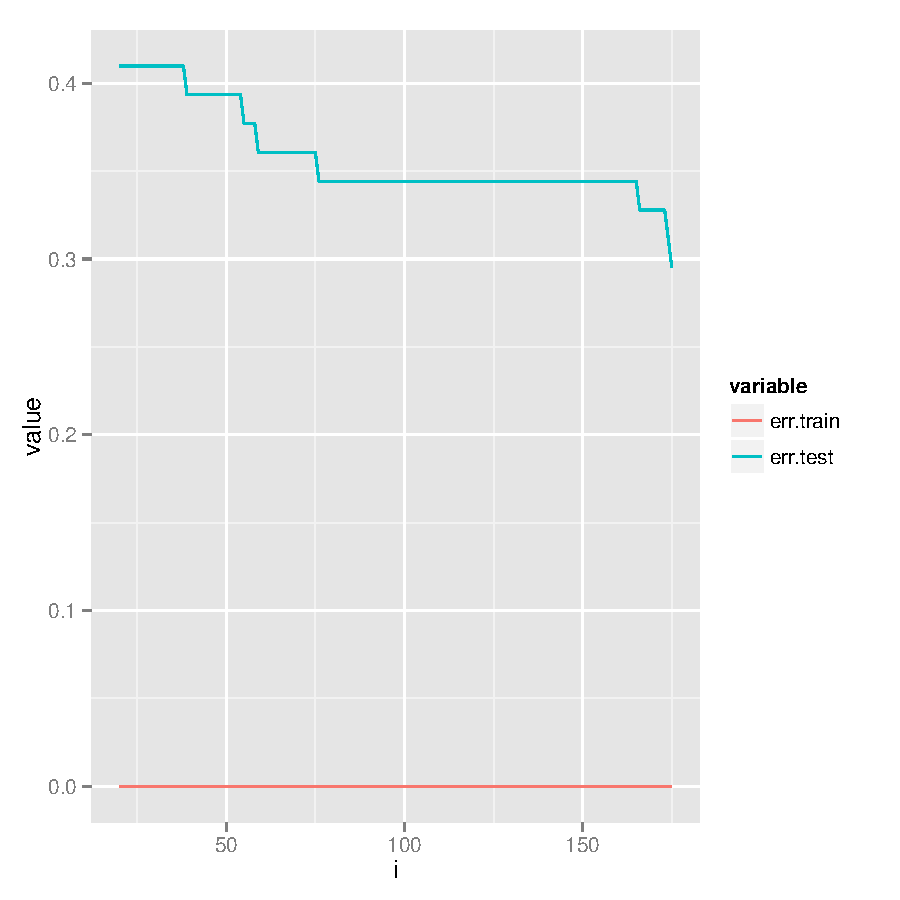
\includegraphics{Final-011}

En esta gráfica podemos observar que las curvas de entrenamiento y validación se encuentran separadas y existe una tendencia de la curva de validación a la baja. Esto sugiere que nuestro error es producto de varianza y que necesitamos obtener una muestra de mayor tamaño para reducir el error.

\subsection{Bosques Aleatorios}
Por último estudiamos el procedimiento de bosques aleatorios. En este caso, en cada experimento entrenamos un bosque formado por 350 árboles que discriminan los datos utilizando el criterio de máxima entropía (\emph{maxEnt}).

De nueva cuenta utilizamos validación cruzada en 5 iteraciones para estimar el error promedio y desviación estándar de la tasa de clasificación del bosque.

\begin{Schunk}
\begin{Sinput}
> tree.cross.validation <- sapply(seq(1,5), function(i){
+   train <- datos.red[unlist(kfolds[c(-i)]),]
+   test <- datos.red[kfolds[[i]],]
+   rf <- randomForest(tipo~.,data=train, ntree=350, importance=TRUE)
+   preds <- predict(rf, newdata = test)
+   mean(preds == test$tipo)
+ })
> m.tree <- mean(tree.cross.validation)
> m.tree
\end{Sinput}
\begin{Soutput}
[1] 0.872961
\end{Soutput}
\begin{Sinput}
> sd.tree <- sd(tree.cross.validation)
> sd.tree
\end{Sinput}
\begin{Soutput}
[1] 0.06705111
\end{Soutput}
\end{Schunk}

Encontramos que en promedio el bosque aleatorio tendrá una tasa media de clasificación del 87.2960992907801\% con una variación de 0.0670511139444611 puntos.

La siguiente figura muestra el comportamiento del bosque aleatorio en las dos componentes principales más importantes.

\begin{Schunk}
\begin{Sinput}
> rf.opt.2 <- randomForest(tipo ~ Comp.1 + Comp.2, 
+                          data = datos.red,
+                          ntree = 350,
+                          importance=TRUE)
> dat.x$preds.rf <- predict(rf.opt.2, newdata = dat.x)
> ggplot(dat.x, aes(x = Comp.1,
+                   y = Comp.2,
+                   colour = preds.rf)) + 
+   geom_point(size = 1) + geom_point(aes(x = Comp.1,
+                                         y = Comp.2,
+                                         color = tipo),
+                                     data = datos.red,
+                                     size = 3) + 
+   xlim(-30,30) + ylim(-20,20)
\end{Sinput}
\end{Schunk}
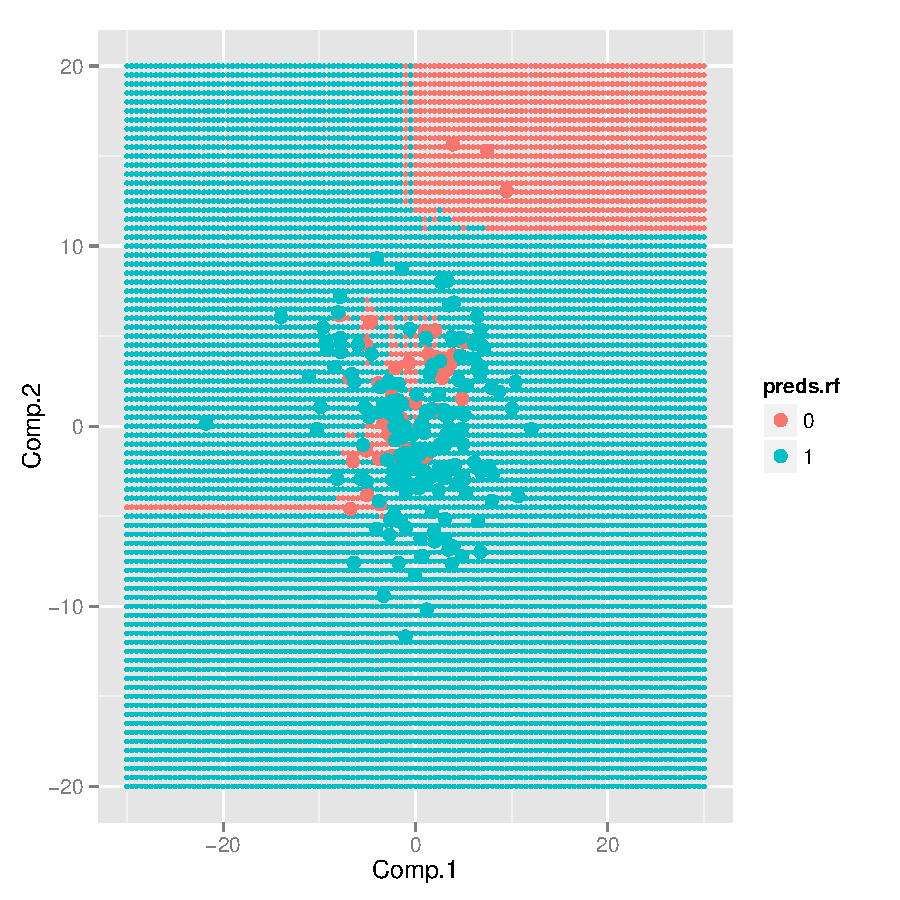
\includegraphics{Final-013}

\subsubsection{Sensibilidad, Precisión y score F1}
Para hacer posible una comparación sobre los modelos, calculamos las mismas métricas que en la sección anterior sobre el mismo conjunto de datos utilizado por el SVM. La matriz de confusión para el bosque aleatorio está dada por 
\begin{Schunk}
\begin{Sinput}
> rf.opt <- randomForest(tipo ~ ., data = train, importance = TRUE)
> preds.opt <- predict(rf.opt, newdata = test)
> t.confusion <- table(preds.opt, test$tipo, deparse.level = 2)
> t.confusion
\end{Sinput}
\begin{Soutput}
         test$tipo
preds.opt  0  1
        0 11  3
        1 15 32
\end{Soutput}
\end{Schunk}

Mientras que las medidas de precisión, sensibilidad y el score F1 son
\begin{Schunk}
\begin{Sinput}
> prec.rf <- t.confusion[1] / (t.confusion[1] + t.confusion[3])
> prec.rf
\end{Sinput}
\begin{Soutput}
[1] 0.7857143
\end{Soutput}
\begin{Sinput}
> recall.rf <- t.confusion[1] / (t.confusion[1] + t.confusion[2])
> recall.rf
\end{Sinput}
\begin{Soutput}
[1] 0.4230769
\end{Soutput}
\begin{Sinput}
> f1.rf <- 2 * (prec.svm * recall.svm) / (prec.svm + recall.svm)
> f1.rf
\end{Sinput}
\begin{Soutput}
[1] 0.4705882
\end{Soutput}
\end{Schunk}

\subsubsection{Sesgo y Varianza del modelo}
Por último, investigamos las maneras en que podemos mejorar el modelo de bosque aleatorio midiendo el error de entrenamiento y prueba a distintos tamaños de muestras.

\begin{Schunk}
\begin{Sinput}
> errs <- sapply(seq(20, dim(train)[1]), function(i){
+   rf.opt <- randomForest(tipo ~ ., data = train[1:i,])
+   #Err train
+   preds.train <- predict(rf.opt, newdata = train[1:i,])
+   err.train <- mean(preds.train != train[1:i,]$tipo)
+   #Err test
+   preds.test <- predict(rf.opt, newdata = test)
+   err.test <- mean(preds.test != test$tipo)
+   list(i, err.train, err.test)
+ })
> errs <- t(errs)
> errs.df.m<- melt(data.frame(i = unlist(errs[,1]),
+                             err.train = unlist(errs[,2]), 
+                             err.test = unlist(errs[,3])), 
+                  id=c("i"))
> ggplot(aes(x = i, 
+            y = value, 
+            colour=variable), 
+        data = errs.df.m) + geom_line()
\end{Sinput}
\end{Schunk}
De nueva cuenta vemos una tendencia del error de validación a la baja, y una diferencia notable entre el error de entrenamiento y el error de prueba. Esto nos da indicación de que el modelo mejoraría si obtuviéramos más pruebas de entrenamiento.


\section{Conclusiones}
De acuerdo a sus características, podemos plantear el problema de distinguir dos tipos de alacranes: no-venenosos y venenosos. A partir de una serie de medidas, se obtuvieron 236 observaciones sobre un espacio de 140 variables. Mediante el procedimiento de análisis de componentes principales, podemos reducir el espacio de variables a sólo 40 acumulando un 97\% de la varianza total, aunque en el transcurso de este trabajo no hubo necesidad pues los algoritmos elegidos corrían sin problema alguno en la totalidad de los datos.
Comparamos dos distintos métodos de clasificación: Máquinas de soporte vectorial y Bosques Aleatorios. Mediante validación cruzada de 5 iteraciones obtuvimos las principales métricas para comparar estos algoritmos. La tabla \ref{tbl:compMod} muestra la comparación.

\begin{table}
  \centering
  \caption{Comparación de las principales métricas de los modelos}
  \begin{tabular}{|c|c|c|c|}
    \hline
    & \textbf{Precisión} & \textbf{Sensibilidad} & \textbf{F1}\\
    \hline
    SVM & 1 & 0.307692307692308 & 0.470588235294118\\
    \hline
    R.F. & 0.785714285714286 & 0.423076923076923 & 0.470588235294118\\
    \hline
  \end{tabular}
  \label{tbl:compMod}
\end{table}

Es interesante notar que ambos modelos tienen el mismo score F1, pero varían en precisión y sensibilidad. 

Utilizando un análisis de sesgo y varianza encontramos que ambos modelos se podrían mejorar si obtenemos una muestra mucho más grande, ya que se notó una tendencia del error de prueba hacia la baja y una separación muy amplia entre el error de validación y el de entrenamiento.

\subsection{?`Qué modelo es mejor?}
Para distinguir los modelos consideremos un ejemplo. Tenemos un alacrán del cual no sabemos si es venenoso o no. Supongamos que se lo presentamos a nuestro modelo y este asegura que no es peligroso. Si en realidad el arácnido era venenoso, nuestro modelo habrá puesto en riesgo nuestra salud. En cambio, si el modelo dice que es venenoso pero en realidad no lo era, no pasa de que nos preocupemos un poco y que nos toque una inyección que no correspondía. El primer error se conoce como el error tipo II y al segundo como tipo I.

De esta manera, queremos elegir el modelo que minimice el error tipo II. Para el tamaño de muestra obtenido hasta el momento, el modelo con menor tasa de error del tipo II es el SVM ya que no asigna ningún alacrán venenoso a la categoría de no peligrosos mientras que el bosque aleatorio tiene 3 fallas. Estos resultados resultan muy débiles y faltaría volver a medir con una muestra más grande.

\end{document}
